\documentclass[twoside]{book}

% Packages required by doxygen
\usepackage{fixltx2e}
\usepackage{calc}
\usepackage{doxygen}
\usepackage[export]{adjustbox} % also loads graphicx
\usepackage{graphicx}
\usepackage[utf8]{inputenc}
\usepackage{makeidx}
\usepackage{multicol}
\usepackage{multirow}
\PassOptionsToPackage{warn}{textcomp}
\usepackage{textcomp}
\usepackage[nointegrals]{wasysym}
\usepackage[table]{xcolor}

% Font selection
\usepackage[T1]{fontenc}
\usepackage[scaled=.90]{helvet}
\usepackage{courier}
\usepackage{amssymb}
\usepackage{sectsty}
\renewcommand{\familydefault}{\sfdefault}
\allsectionsfont{%
  \fontseries{bc}\selectfont%
  \color{darkgray}%
}
\renewcommand{\DoxyLabelFont}{%
  \fontseries{bc}\selectfont%
  \color{darkgray}%
}
\newcommand{\+}{\discretionary{\mbox{\scriptsize$\hookleftarrow$}}{}{}}

% Page & text layout
\usepackage{geometry}
\geometry{%
  a4paper,%
  top=2.5cm,%
  bottom=2.5cm,%
  left=2.5cm,%
  right=2.5cm%
}
\tolerance=750
\hfuzz=15pt
\hbadness=750
\setlength{\emergencystretch}{15pt}
\setlength{\parindent}{0cm}
\setlength{\parskip}{3ex plus 2ex minus 2ex}
\makeatletter
\renewcommand{\paragraph}{%
  \@startsection{paragraph}{4}{0ex}{-1.0ex}{1.0ex}{%
    \normalfont\normalsize\bfseries\SS@parafont%
  }%
}
\renewcommand{\subparagraph}{%
  \@startsection{subparagraph}{5}{0ex}{-1.0ex}{1.0ex}{%
    \normalfont\normalsize\bfseries\SS@subparafont%
  }%
}
\makeatother

% Headers & footers
\usepackage{fancyhdr}
\pagestyle{fancyplain}
\fancyhead[LE]{\fancyplain{}{\bfseries\thepage}}
\fancyhead[CE]{\fancyplain{}{}}
\fancyhead[RE]{\fancyplain{}{\bfseries\leftmark}}
\fancyhead[LO]{\fancyplain{}{\bfseries\rightmark}}
\fancyhead[CO]{\fancyplain{}{}}
\fancyhead[RO]{\fancyplain{}{\bfseries\thepage}}
\fancyfoot[LE]{\fancyplain{}{}}
\fancyfoot[CE]{\fancyplain{}{}}
\fancyfoot[RE]{\fancyplain{}{\bfseries\scriptsize Generated by Doxygen }}
\fancyfoot[LO]{\fancyplain{}{\bfseries\scriptsize Generated by Doxygen }}
\fancyfoot[CO]{\fancyplain{}{}}
\fancyfoot[RO]{\fancyplain{}{}}
\renewcommand{\footrulewidth}{0.4pt}
\renewcommand{\chaptermark}[1]{%
  \markboth{#1}{}%
}
\renewcommand{\sectionmark}[1]{%
  \markright{\thesection\ #1}%
}

% Indices & bibliography
\usepackage{natbib}
\usepackage[titles]{tocloft}
\setcounter{tocdepth}{3}
\setcounter{secnumdepth}{5}
\makeindex

% Hyperlinks (required, but should be loaded last)
\usepackage{ifpdf}
\ifpdf
  \usepackage[pdftex,pagebackref=true]{hyperref}
\else
  \usepackage[ps2pdf,pagebackref=true]{hyperref}
\fi
\hypersetup{%
  colorlinks=true,%
  linkcolor=blue,%
  citecolor=blue,%
  unicode%
}

% Custom commands
\newcommand{\clearemptydoublepage}{%
  \newpage{\pagestyle{empty}\cleardoublepage}%
}

\usepackage{caption}
\captionsetup{labelsep=space,justification=centering,font={bf},singlelinecheck=off,skip=4pt,position=top}

%===== C O N T E N T S =====

\begin{document}

% Titlepage & ToC
\hypersetup{pageanchor=false,
             bookmarksnumbered=true,
             pdfencoding=unicode
            }
\pagenumbering{alph}
\begin{titlepage}
\vspace*{7cm}
\begin{center}%
{\Large My Project }\\
\vspace*{1cm}
{\large Generated by Doxygen 1.8.13}\\
\end{center}
\end{titlepage}
\clearemptydoublepage
\pagenumbering{roman}
\tableofcontents
\clearemptydoublepage
\pagenumbering{arabic}
\hypersetup{pageanchor=true}

%--- Begin generated contents ---
\chapter{cop290}
\label{md_README}
\Hypertarget{md_README}
\section*{cop290}
\chapter{readme}
\label{md_readme}
\Hypertarget{md_readme}
We have made several modules, description is as follows.
\begin{DoxyItemize}
\item \hyperlink{input_8cpp}{input.\+cpp} -\/ handles all input related
\item \hyperlink{matrices_8cpp}{matrices.\+cpp} -\/ handles all matrix operations that would be required
\item \hyperlink{Output_8cpp}{Output.\+cpp} -\/ handles all output related
\item \hyperlink{threeD__to__ortho_8cpp}{three\+D\+\_\+to\+\_\+ortho.\+cpp} -\/ handles all 3D to 2D transformation
\item \hyperlink{twoD__to__threeD_8cpp}{two\+D\+\_\+to\+\_\+three\+D.\+cpp} -\/ handles all 2D to 3D transformations 
\end{DoxyItemize}
\chapter{Class Index}
\section{Class List}
Here are the classes, structs, unions and interfaces with brief descriptions\+:\begin{DoxyCompactList}
\item\contentsline{section}{\hyperlink{structcoordinate}{coordinate} }{\pageref{structcoordinate}}{}
\item\contentsline{section}{\hyperlink{structdir__ratios}{dir\+\_\+ratios} }{\pageref{structdir__ratios}}{}
\item\contentsline{section}{\hyperlink{structdirection}{direction} }{\pageref{structdirection}}{}
\item\contentsline{section}{\hyperlink{structedge}{edge} }{\pageref{structedge}}{}
\item\contentsline{section}{\hyperlink{structgraph}{graph} }{\pageref{structgraph}}{}
\item\contentsline{section}{\hyperlink{classMainWindow}{Main\+Window} }{\pageref{classMainWindow}}{}
\item\contentsline{section}{\hyperlink{structnode}{node} }{\pageref{structnode}}{}
\item\contentsline{section}{\hyperlink{structpair__}{pair\+\_\+} }{\pageref{structpair__}}{}
\item\contentsline{section}{\hyperlink{classQMainWindow}{Q\+Main\+Window} }{\pageref{classQMainWindow}}{}
\item\contentsline{section}{\hyperlink{structrot__matrix}{rot\+\_\+matrix} }{\pageref{structrot__matrix}}{}
\item\contentsline{section}{\hyperlink{structthreeView}{three\+View} }{\pageref{structthreeView}}{}
\end{DoxyCompactList}

\chapter{File Index}
\section{File List}
Here is a list of all files with brief descriptions\+:\begin{DoxyCompactList}
\item\contentsline{section}{\hyperlink{draw_8cpp}{draw.\+cpp} }{\pageref{draw_8cpp}}{}
\item\contentsline{section}{\hyperlink{input_8cpp}{input.\+cpp} }{\pageref{input_8cpp}}{}
\item\contentsline{section}{\hyperlink{main_8cpp}{main.\+cpp} }{\pageref{main_8cpp}}{}
\item\contentsline{section}{\hyperlink{mainwindow_8cpp}{mainwindow.\+cpp} }{\pageref{mainwindow_8cpp}}{}
\item\contentsline{section}{\hyperlink{mainwindow_8h}{mainwindow.\+h} }{\pageref{mainwindow_8h}}{}
\item\contentsline{section}{\hyperlink{struct_8h}{struct.\+h} }{\pageref{struct_8h}}{}
\item\contentsline{section}{\hyperlink{threeD__to__ortho_8cpp}{three\+D\+\_\+to\+\_\+ortho.\+cpp} }{\pageref{threeD__to__ortho_8cpp}}{}
\item\contentsline{section}{\hyperlink{twoD__to3D_8cpp}{two\+D\+\_\+to3\+D.\+cpp} }{\pageref{twoD__to3D_8cpp}}{}
\end{DoxyCompactList}

\chapter{Class Documentation}
\hypertarget{structadjacency__list}{}\section{adjacency\+\_\+list Struct Reference}
\label{structadjacency__list}\index{adjacency\+\_\+list@{adjacency\+\_\+list}}


Collaboration diagram for adjacency\+\_\+list\+:
% FIG 0
\subsection*{Public Attributes}
\begin{DoxyCompactItemize}
\item 
vector$<$ \hyperlink{structcoordinates}{coordinates} $>$ \hyperlink{structadjacency__list_a1597c7524394cfee124109aadd4efe4a}{adj\+\_\+list}
\item 
\hyperlink{structcoordinates}{coordinates} \hyperlink{structadjacency__list_aa1879f5cdc8b59e3ce1998aa93645dcf}{coord}
\end{DoxyCompactItemize}


\subsection{Member Data Documentation}
\mbox{\Hypertarget{structadjacency__list_a1597c7524394cfee124109aadd4efe4a}\label{structadjacency__list_a1597c7524394cfee124109aadd4efe4a}} 
\index{adjacency\+\_\+list@{adjacency\+\_\+list}!adj\+\_\+list@{adj\+\_\+list}}
\index{adj\+\_\+list@{adj\+\_\+list}!adjacency\+\_\+list@{adjacency\+\_\+list}}
\subsubsection{\texorpdfstring{adj\+\_\+list}{adj\_list}}
{\footnotesize\ttfamily vector$<$\hyperlink{structcoordinates}{coordinates}$>$ adjacency\+\_\+list\+::adj\+\_\+list}

\mbox{\Hypertarget{structadjacency__list_aa1879f5cdc8b59e3ce1998aa93645dcf}\label{structadjacency__list_aa1879f5cdc8b59e3ce1998aa93645dcf}} 
\index{adjacency\+\_\+list@{adjacency\+\_\+list}!coord@{coord}}
\index{coord@{coord}!adjacency\+\_\+list@{adjacency\+\_\+list}}
\subsubsection{\texorpdfstring{coord}{coord}}
{\footnotesize\ttfamily \hyperlink{structcoordinates}{coordinates} adjacency\+\_\+list\+::coord}



The documentation for this struct was generated from the following file\+:\begin{DoxyCompactItemize}
\item 
\hyperlink{input_8cpp}{input.\+cpp}\end{DoxyCompactItemize}

\hypertarget{structcoordinates}{}\section{coordinates Struct Reference}
\label{structcoordinates}\index{coordinates@{coordinates}}


Collaboration diagram for coordinates\+:
% FIG 0
\subsection*{Public Attributes}
\begin{DoxyCompactItemize}
\item 
int \hyperlink{structcoordinates_a1047b469a6d5827293066e71649b9acc}{x}
\item 
int \hyperlink{structcoordinates_af7fe5145df74388a36fd7b283992e9a5}{y}
\item 
int \hyperlink{structcoordinates_a1adf14ce5b540ddde151c5bfe04b2cd8}{z}
\end{DoxyCompactItemize}


\subsection{Member Data Documentation}
\mbox{\Hypertarget{structcoordinates_a1047b469a6d5827293066e71649b9acc}\label{structcoordinates_a1047b469a6d5827293066e71649b9acc}} 
\index{coordinates@{coordinates}!x@{x}}
\index{x@{x}!coordinates@{coordinates}}
\subsubsection{\texorpdfstring{x}{x}}
{\footnotesize\ttfamily int coordinates\+::x}

\mbox{\Hypertarget{structcoordinates_af7fe5145df74388a36fd7b283992e9a5}\label{structcoordinates_af7fe5145df74388a36fd7b283992e9a5}} 
\index{coordinates@{coordinates}!y@{y}}
\index{y@{y}!coordinates@{coordinates}}
\subsubsection{\texorpdfstring{y}{y}}
{\footnotesize\ttfamily int coordinates\+::y}

\mbox{\Hypertarget{structcoordinates_a1adf14ce5b540ddde151c5bfe04b2cd8}\label{structcoordinates_a1adf14ce5b540ddde151c5bfe04b2cd8}} 
\index{coordinates@{coordinates}!z@{z}}
\index{z@{z}!coordinates@{coordinates}}
\subsubsection{\texorpdfstring{z}{z}}
{\footnotesize\ttfamily int coordinates\+::z}



The documentation for this struct was generated from the following file\+:\begin{DoxyCompactItemize}
\item 
\hyperlink{input_8cpp}{input.\+cpp}\end{DoxyCompactItemize}

\hypertarget{structgraph}{}\section{graph Struct Reference}
\label{structgraph}\index{graph@{graph}}


Collaboration diagram for graph\+:
% FIG 0
\subsection*{Public Attributes}
\begin{DoxyCompactItemize}
\item 
vector$<$ \hyperlink{structadjacency__list}{adjacency\+\_\+list} $>$ \hyperlink{structgraph_ad0db17a95ef55e60b39b28fa2f11447c}{g}
\end{DoxyCompactItemize}


\subsection{Member Data Documentation}
\mbox{\Hypertarget{structgraph_ad0db17a95ef55e60b39b28fa2f11447c}\label{structgraph_ad0db17a95ef55e60b39b28fa2f11447c}} 
\index{graph@{graph}!g@{g}}
\index{g@{g}!graph@{graph}}
\subsubsection{\texorpdfstring{g}{g}}
{\footnotesize\ttfamily vector$<$\hyperlink{structadjacency__list}{adjacency\+\_\+list}$>$ graph\+::g}



The documentation for this struct was generated from the following file\+:\begin{DoxyCompactItemize}
\item 
\hyperlink{input_8cpp}{input.\+cpp}\end{DoxyCompactItemize}

\hypertarget{classinput}{}\section{input Class Reference}
\label{classinput}\index{input@{input}}


Collaboration diagram for input\+:
% FIG 0
\subsection*{Public Member Functions}
\begin{DoxyCompactItemize}
\item 
int \hyperlink{classinput_a09da13fb41c30064a99da7776c0af0e6}{select\+\_\+mode} ()
\item 
void \hyperlink{classinput_aa8115a97b7b36912fd20a24fba00f0cc}{get\+\_\+input} ()
\item 
\hyperlink{structgraph}{graph} \hyperlink{classinput_aa48aa4244183a1c9638307d13caeeeea}{three\+D\+\_\+to\+\_\+graph} ()
\item 
\hyperlink{structgraph}{graph} \hyperlink{classinput_a42bcdd5bfcccd4cab629d115cd56a846}{two\+D\+\_\+to\+\_\+graph} ()
\end{DoxyCompactItemize}


\subsection{Member Function Documentation}
\mbox{\Hypertarget{classinput_aa8115a97b7b36912fd20a24fba00f0cc}\label{classinput_aa8115a97b7b36912fd20a24fba00f0cc}} 
\index{input@{input}!get\+\_\+input@{get\+\_\+input}}
\index{get\+\_\+input@{get\+\_\+input}!input@{input}}
\subsubsection{\texorpdfstring{get\+\_\+input()}{get\_input()}}
{\footnotesize\ttfamily void input\+::get\+\_\+input (\begin{DoxyParamCaption}{ }\end{DoxyParamCaption})\hspace{0.3cm}{\ttfamily [inline]}}

Fetches the input file and validates the format in accordance with the mode seleted by the user.\mbox{\Hypertarget{classinput_a09da13fb41c30064a99da7776c0af0e6}\label{classinput_a09da13fb41c30064a99da7776c0af0e6}} 
\index{input@{input}!select\+\_\+mode@{select\+\_\+mode}}
\index{select\+\_\+mode@{select\+\_\+mode}!input@{input}}
\subsubsection{\texorpdfstring{select\+\_\+mode()}{select\_mode()}}
{\footnotesize\ttfamily int input\+::select\+\_\+mode (\begin{DoxyParamCaption}{ }\end{DoxyParamCaption})\hspace{0.3cm}{\ttfamily [inline]}}

Asks the user to choose the mode of operation out of the following\+:
\begin{DoxyEnumerate}
\item 3D input to orthographic views or
\item 2D orthographic views as input to generate isometric views.
\end{DoxyEnumerate}\mbox{\Hypertarget{classinput_aa48aa4244183a1c9638307d13caeeeea}\label{classinput_aa48aa4244183a1c9638307d13caeeeea}} 
\index{input@{input}!three\+D\+\_\+to\+\_\+graph@{three\+D\+\_\+to\+\_\+graph}}
\index{three\+D\+\_\+to\+\_\+graph@{three\+D\+\_\+to\+\_\+graph}!input@{input}}
\subsubsection{\texorpdfstring{three\+D\+\_\+to\+\_\+graph()}{threeD\_to\_graph()}}
{\footnotesize\ttfamily \hyperlink{structgraph}{graph} input\+::three\+D\+\_\+to\+\_\+graph (\begin{DoxyParamCaption}{ }\end{DoxyParamCaption})\hspace{0.3cm}{\ttfamily [inline]}}

Converts the given 3D input into a graph. Graph is described as follows
\begin{DoxyItemize}
\item Graph is a list of vertices
\item Each vertex itself has a coordinate value associated with itself
\item Each vertex also has an adjacency list that stores the coordinates of its neighbours (i.\+e the vertices with the current vertex shares an edge)
\end{DoxyItemize}\mbox{\Hypertarget{classinput_a42bcdd5bfcccd4cab629d115cd56a846}\label{classinput_a42bcdd5bfcccd4cab629d115cd56a846}} 
\index{input@{input}!two\+D\+\_\+to\+\_\+graph@{two\+D\+\_\+to\+\_\+graph}}
\index{two\+D\+\_\+to\+\_\+graph@{two\+D\+\_\+to\+\_\+graph}!input@{input}}
\subsubsection{\texorpdfstring{two\+D\+\_\+to\+\_\+graph()}{twoD\_to\_graph()}}
{\footnotesize\ttfamily \hyperlink{structgraph}{graph} input\+::two\+D\+\_\+to\+\_\+graph (\begin{DoxyParamCaption}{ }\end{DoxyParamCaption})\hspace{0.3cm}{\ttfamily [inline]}}

Converts the 2D input to a probable 3D graph descriptions according to the following procedure.
\begin{DoxyItemize}
\item Find correspondence of different points in all 3 orthographic views to get the 3D description of the vertices in the 3D model.
\item Find and add all the probable edges to the graph formed in last step.
\item Check for the presence of redundant edges and vertices in the graph formed.
\item Get orthographic views of the graph generated and match with the initial input orthographic views.
\item If the views match then the graph is the final description of the 3D model.
\item Else check again for redundancy until the views match with each other.
\end{DoxyItemize}

The documentation for this class was generated from the following file\+:\begin{DoxyCompactItemize}
\item 
\hyperlink{input_8cpp}{input.\+cpp}\end{DoxyCompactItemize}

\hypertarget{classmatrices}{}\section{matrices Class Reference}
\label{classmatrices}\index{matrices@{matrices}}


Collaboration diagram for matrices\+:
% FIG 0
\subsection*{Public Member Functions}
\begin{DoxyCompactItemize}
\item 
int $\ast$ \hyperlink{classmatrices_a65e362b1db7ec3bf04b60b868e8b432d}{add4x4} (int arr\mbox{[}$\,$\mbox{]}\mbox{[}$\,$\mbox{]})
\item 
int $\ast$ \hyperlink{classmatrices_a97708324cbb5612c867c494846116c84}{mult4x4} (int arr\mbox{[}$\,$\mbox{]}\mbox{[}$\,$\mbox{]})
\item 
int $\ast$ \hyperlink{classmatrices_a1200dc125cabee08728f6bec0aa8905a}{add3x3} (int arr\mbox{[}$\,$\mbox{]}\mbox{[}$\,$\mbox{]})
\item 
int $\ast$ \hyperlink{classmatrices_a23a1caa682ac0fb8941e6f5a4cfd6cb7}{mult3x3} (int arr\mbox{[}$\,$\mbox{]}\mbox{[}$\,$\mbox{]})
\end{DoxyCompactItemize}


\subsection{Member Function Documentation}
\mbox{\Hypertarget{classmatrices_a1200dc125cabee08728f6bec0aa8905a}\label{classmatrices_a1200dc125cabee08728f6bec0aa8905a}} 
\index{matrices@{matrices}!add3x3@{add3x3}}
\index{add3x3@{add3x3}!matrices@{matrices}}
\subsubsection{\texorpdfstring{add3x3()}{add3x3()}}
{\footnotesize\ttfamily int$\ast$ matrices\+::add3x3 (\begin{DoxyParamCaption}\item[{int}]{arr\mbox{[}$\,$\mbox{]}\mbox{[}$\,$\mbox{]} }\end{DoxyParamCaption})\hspace{0.3cm}{\ttfamily [inline]}}

\mbox{\Hypertarget{classmatrices_a65e362b1db7ec3bf04b60b868e8b432d}\label{classmatrices_a65e362b1db7ec3bf04b60b868e8b432d}} 
\index{matrices@{matrices}!add4x4@{add4x4}}
\index{add4x4@{add4x4}!matrices@{matrices}}
\subsubsection{\texorpdfstring{add4x4()}{add4x4()}}
{\footnotesize\ttfamily int$\ast$ matrices\+::add4x4 (\begin{DoxyParamCaption}\item[{int}]{arr\mbox{[}$\,$\mbox{]}\mbox{[}$\,$\mbox{]} }\end{DoxyParamCaption})\hspace{0.3cm}{\ttfamily [inline]}}

\mbox{\Hypertarget{classmatrices_a23a1caa682ac0fb8941e6f5a4cfd6cb7}\label{classmatrices_a23a1caa682ac0fb8941e6f5a4cfd6cb7}} 
\index{matrices@{matrices}!mult3x3@{mult3x3}}
\index{mult3x3@{mult3x3}!matrices@{matrices}}
\subsubsection{\texorpdfstring{mult3x3()}{mult3x3()}}
{\footnotesize\ttfamily int$\ast$ matrices\+::mult3x3 (\begin{DoxyParamCaption}\item[{int}]{arr\mbox{[}$\,$\mbox{]}\mbox{[}$\,$\mbox{]} }\end{DoxyParamCaption})\hspace{0.3cm}{\ttfamily [inline]}}

\mbox{\Hypertarget{classmatrices_a97708324cbb5612c867c494846116c84}\label{classmatrices_a97708324cbb5612c867c494846116c84}} 
\index{matrices@{matrices}!mult4x4@{mult4x4}}
\index{mult4x4@{mult4x4}!matrices@{matrices}}
\subsubsection{\texorpdfstring{mult4x4()}{mult4x4()}}
{\footnotesize\ttfamily int$\ast$ matrices\+::mult4x4 (\begin{DoxyParamCaption}\item[{int}]{arr\mbox{[}$\,$\mbox{]}\mbox{[}$\,$\mbox{]} }\end{DoxyParamCaption})\hspace{0.3cm}{\ttfamily [inline]}}



The documentation for this class was generated from the following file\+:\begin{DoxyCompactItemize}
\item 
\hyperlink{matrices_8cpp}{matrices.\+cpp}\end{DoxyCompactItemize}

\hypertarget{classOutput}{}\section{Output Class Reference}
\label{classOutput}\index{Output@{Output}}


Collaboration diagram for Output\+:
% FIG 0
\subsection*{Public Member Functions}
\begin{DoxyCompactItemize}
\item 
bool \hyperlink{classOutput_af1d58420785a9c9601c6888df473fc96}{save\+\_\+or\+\_\+not} ()
\item 
string \hyperlink{classOutput_a0df9c8e902530f9839ef0a31f7a4e42d}{Output\+\_\+file\+\_\+name} ()
\item 
void \hyperlink{classOutput_add61bdc5030a63a127ad67e70288a3e9}{save\+\_\+output} (bool \hyperlink{classOutput_af1d58420785a9c9601c6888df473fc96}{save\+\_\+or\+\_\+not}, string \hyperlink{classOutput_a0df9c8e902530f9839ef0a31f7a4e42d}{Output\+\_\+file\+\_\+name})
\end{DoxyCompactItemize}


\subsection{Member Function Documentation}
\mbox{\Hypertarget{classOutput_a0df9c8e902530f9839ef0a31f7a4e42d}\label{classOutput_a0df9c8e902530f9839ef0a31f7a4e42d}} 
\index{Output@{Output}!Output\+\_\+file\+\_\+name@{Output\+\_\+file\+\_\+name}}
\index{Output\+\_\+file\+\_\+name@{Output\+\_\+file\+\_\+name}!Output@{Output}}
\subsubsection{\texorpdfstring{Output\+\_\+file\+\_\+name()}{Output\_file\_name()}}
{\footnotesize\ttfamily string Output\+::\+Output\+\_\+file\+\_\+name (\begin{DoxyParamCaption}{ }\end{DoxyParamCaption})\hspace{0.3cm}{\ttfamily [inline]}}

Asks user the name which the user desires to give to the \hyperlink{classOutput}{Output} file.\mbox{\Hypertarget{classOutput_af1d58420785a9c9601c6888df473fc96}\label{classOutput_af1d58420785a9c9601c6888df473fc96}} 
\index{Output@{Output}!save\+\_\+or\+\_\+not@{save\+\_\+or\+\_\+not}}
\index{save\+\_\+or\+\_\+not@{save\+\_\+or\+\_\+not}!Output@{Output}}
\subsubsection{\texorpdfstring{save\+\_\+or\+\_\+not()}{save\_or\_not()}}
{\footnotesize\ttfamily bool Output\+::save\+\_\+or\+\_\+not (\begin{DoxyParamCaption}{ }\end{DoxyParamCaption})\hspace{0.3cm}{\ttfamily [inline]}}

Asks user if he/she desires to save the output file that has been generated.\mbox{\Hypertarget{classOutput_add61bdc5030a63a127ad67e70288a3e9}\label{classOutput_add61bdc5030a63a127ad67e70288a3e9}} 
\index{Output@{Output}!save\+\_\+output@{save\+\_\+output}}
\index{save\+\_\+output@{save\+\_\+output}!Output@{Output}}
\subsubsection{\texorpdfstring{save\+\_\+output()}{save\_output()}}
{\footnotesize\ttfamily void Output\+::save\+\_\+output (\begin{DoxyParamCaption}\item[{bool}]{save\+\_\+or\+\_\+not,  }\item[{string}]{Output\+\_\+file\+\_\+name }\end{DoxyParamCaption})\hspace{0.3cm}{\ttfamily [inline]}}

Checks if the user wants to save the output Saves the output generated in the corresponding format with the file name specified by the user.

The documentation for this class was generated from the following file\+:\begin{DoxyCompactItemize}
\item 
\hyperlink{Output_8cpp}{Output.\+cpp}\end{DoxyCompactItemize}

\hypertarget{classthreeD__to__ortho}{}\section{three\+D\+\_\+to\+\_\+ortho Class Reference}
\label{classthreeD__to__ortho}\index{three\+D\+\_\+to\+\_\+ortho@{three\+D\+\_\+to\+\_\+ortho}}


Collaboration diagram for three\+D\+\_\+to\+\_\+ortho\+:
% FIG 0
\subsection*{Public Member Functions}
\begin{DoxyCompactItemize}
\item 
void \hyperlink{classthreeD__to__ortho_a3d16f355dc29a6de3073700246a50fc0}{translate\+\_\+coordinate} (coordinate c1, coordinate c2)
\item 
void \hyperlink{classthreeD__to__ortho_a721cf3d866a5b6abf941c726fca3cadc}{translate\+\_\+graph} (\hyperlink{structgraph}{graph} g, coordinate c)
\item 
void \hyperlink{classthreeD__to__ortho_aee77836500d9b77c9485fd782496d91b}{get\+\_\+direction\+\_\+for\+\_\+projection} ()
\item 
void \hyperlink{classthreeD__to__ortho_a14f6162b721d0f59aec4b08b38e45212}{rotate} ()
\item 
void \hyperlink{classthreeD__to__ortho_a566486a4d1907f4fef666fc2df837786}{projection} ()
\item 
void \hyperlink{classthreeD__to__ortho_a755b7a3d0121bb909a2a564e1b192bf6}{get\+\_\+transitions} ()
\item 
void \hyperlink{classthreeD__to__ortho_af25b29a601ee4b49c3db58ac6e96126c}{make\+\_\+transitions} ()
\end{DoxyCompactItemize}


\subsection{Member Function Documentation}
\mbox{\Hypertarget{classthreeD__to__ortho_aee77836500d9b77c9485fd782496d91b}\label{classthreeD__to__ortho_aee77836500d9b77c9485fd782496d91b}} 
\index{three\+D\+\_\+to\+\_\+ortho@{three\+D\+\_\+to\+\_\+ortho}!get\+\_\+direction\+\_\+for\+\_\+projection@{get\+\_\+direction\+\_\+for\+\_\+projection}}
\index{get\+\_\+direction\+\_\+for\+\_\+projection@{get\+\_\+direction\+\_\+for\+\_\+projection}!three\+D\+\_\+to\+\_\+ortho@{three\+D\+\_\+to\+\_\+ortho}}
\subsubsection{\texorpdfstring{get\+\_\+direction\+\_\+for\+\_\+projection()}{get\_direction\_for\_projection()}}
{\footnotesize\ttfamily void three\+D\+\_\+to\+\_\+ortho\+::get\+\_\+direction\+\_\+for\+\_\+projection (\begin{DoxyParamCaption}{ }\end{DoxyParamCaption})\hspace{0.3cm}{\ttfamily [inline]}}

\mbox{\Hypertarget{classthreeD__to__ortho_a755b7a3d0121bb909a2a564e1b192bf6}\label{classthreeD__to__ortho_a755b7a3d0121bb909a2a564e1b192bf6}} 
\index{three\+D\+\_\+to\+\_\+ortho@{three\+D\+\_\+to\+\_\+ortho}!get\+\_\+transitions@{get\+\_\+transitions}}
\index{get\+\_\+transitions@{get\+\_\+transitions}!three\+D\+\_\+to\+\_\+ortho@{three\+D\+\_\+to\+\_\+ortho}}
\subsubsection{\texorpdfstring{get\+\_\+transitions()}{get\_transitions()}}
{\footnotesize\ttfamily void three\+D\+\_\+to\+\_\+ortho\+::get\+\_\+transitions (\begin{DoxyParamCaption}{ }\end{DoxyParamCaption})\hspace{0.3cm}{\ttfamily [inline]}}

\mbox{\Hypertarget{classthreeD__to__ortho_af25b29a601ee4b49c3db58ac6e96126c}\label{classthreeD__to__ortho_af25b29a601ee4b49c3db58ac6e96126c}} 
\index{three\+D\+\_\+to\+\_\+ortho@{three\+D\+\_\+to\+\_\+ortho}!make\+\_\+transitions@{make\+\_\+transitions}}
\index{make\+\_\+transitions@{make\+\_\+transitions}!three\+D\+\_\+to\+\_\+ortho@{three\+D\+\_\+to\+\_\+ortho}}
\subsubsection{\texorpdfstring{make\+\_\+transitions()}{make\_transitions()}}
{\footnotesize\ttfamily void three\+D\+\_\+to\+\_\+ortho\+::make\+\_\+transitions (\begin{DoxyParamCaption}{ }\end{DoxyParamCaption})\hspace{0.3cm}{\ttfamily [inline]}}

\mbox{\Hypertarget{classthreeD__to__ortho_a566486a4d1907f4fef666fc2df837786}\label{classthreeD__to__ortho_a566486a4d1907f4fef666fc2df837786}} 
\index{three\+D\+\_\+to\+\_\+ortho@{three\+D\+\_\+to\+\_\+ortho}!projection@{projection}}
\index{projection@{projection}!three\+D\+\_\+to\+\_\+ortho@{three\+D\+\_\+to\+\_\+ortho}}
\subsubsection{\texorpdfstring{projection()}{projection()}}
{\footnotesize\ttfamily void three\+D\+\_\+to\+\_\+ortho\+::projection (\begin{DoxyParamCaption}{ }\end{DoxyParamCaption})\hspace{0.3cm}{\ttfamily [inline]}}

\mbox{\Hypertarget{classthreeD__to__ortho_a14f6162b721d0f59aec4b08b38e45212}\label{classthreeD__to__ortho_a14f6162b721d0f59aec4b08b38e45212}} 
\index{three\+D\+\_\+to\+\_\+ortho@{three\+D\+\_\+to\+\_\+ortho}!rotate@{rotate}}
\index{rotate@{rotate}!three\+D\+\_\+to\+\_\+ortho@{three\+D\+\_\+to\+\_\+ortho}}
\subsubsection{\texorpdfstring{rotate()}{rotate()}}
{\footnotesize\ttfamily void three\+D\+\_\+to\+\_\+ortho\+::rotate (\begin{DoxyParamCaption}{ }\end{DoxyParamCaption})\hspace{0.3cm}{\ttfamily [inline]}}

\mbox{\Hypertarget{classthreeD__to__ortho_a3d16f355dc29a6de3073700246a50fc0}\label{classthreeD__to__ortho_a3d16f355dc29a6de3073700246a50fc0}} 
\index{three\+D\+\_\+to\+\_\+ortho@{three\+D\+\_\+to\+\_\+ortho}!translate\+\_\+coordinate@{translate\+\_\+coordinate}}
\index{translate\+\_\+coordinate@{translate\+\_\+coordinate}!three\+D\+\_\+to\+\_\+ortho@{three\+D\+\_\+to\+\_\+ortho}}
\subsubsection{\texorpdfstring{translate\+\_\+coordinate()}{translate\_coordinate()}}
{\footnotesize\ttfamily void three\+D\+\_\+to\+\_\+ortho\+::translate\+\_\+coordinate (\begin{DoxyParamCaption}\item[{coordinate}]{c1,  }\item[{coordinate}]{c2 }\end{DoxyParamCaption})\hspace{0.3cm}{\ttfamily [inline]}}

\mbox{\Hypertarget{classthreeD__to__ortho_a721cf3d866a5b6abf941c726fca3cadc}\label{classthreeD__to__ortho_a721cf3d866a5b6abf941c726fca3cadc}} 
\index{three\+D\+\_\+to\+\_\+ortho@{three\+D\+\_\+to\+\_\+ortho}!translate\+\_\+graph@{translate\+\_\+graph}}
\index{translate\+\_\+graph@{translate\+\_\+graph}!three\+D\+\_\+to\+\_\+ortho@{three\+D\+\_\+to\+\_\+ortho}}
\subsubsection{\texorpdfstring{translate\+\_\+graph()}{translate\_graph()}}
{\footnotesize\ttfamily void three\+D\+\_\+to\+\_\+ortho\+::translate\+\_\+graph (\begin{DoxyParamCaption}\item[{\hyperlink{structgraph}{graph}}]{g,  }\item[{coordinate}]{c }\end{DoxyParamCaption})\hspace{0.3cm}{\ttfamily [inline]}}



The documentation for this class was generated from the following file\+:\begin{DoxyCompactItemize}
\item 
\hyperlink{threeD__to__ortho_8cpp}{three\+D\+\_\+to\+\_\+ortho.\+cpp}\end{DoxyCompactItemize}

\hypertarget{classtwoD__to__threeD}{}\section{two\+D\+\_\+to\+\_\+threeD Class Reference}
\label{classtwoD__to__threeD}\index{two\+D\+\_\+to\+\_\+threeD@{two\+D\+\_\+to\+\_\+threeD}}


Collaboration diagram for two\+D\+\_\+to\+\_\+threeD\+:
% FIG 0
\subsection*{Public Member Functions}
\begin{DoxyCompactItemize}
\item 
returntype \hyperlink{classtwoD__to__threeD_a18411d2d15bff47be2d709dc65681332}{find\+\_\+correspondence} ()
\item 
returntype \hyperlink{classtwoD__to__threeD_a4aa1b891f73475589a3278bf06eb3813}{generate\+\_\+3\+D\+\_\+edges} ()
\item 
returntype \hyperlink{classtwoD__to__threeD_a654dd311058fcb4e155a6f6303605d1d}{generate\+\_\+face} ()
\item 
returntype \hyperlink{classtwoD__to__threeD_abd66b5a812873b0b4694482b26e7698c}{generate\+\_\+3\+D\+\_\+object} ()
\item 
returntype \hyperlink{classtwoD__to__threeD_a6cd16bd23d7f167befdbca13a833be66}{check\+\_\+edges} ()
\item 
returntype \hyperlink{classtwoD__to__threeD_a3e501c816e4c3b6106f1f9190be2975f}{check\+\_\+vertices} ()
\item 
returntype \hyperlink{classtwoD__to__threeD_adee1061487b16954b2596aff1f23999a}{check\+\_\+faces} ()
\end{DoxyCompactItemize}


\subsection{Member Function Documentation}
\mbox{\Hypertarget{classtwoD__to__threeD_a6cd16bd23d7f167befdbca13a833be66}\label{classtwoD__to__threeD_a6cd16bd23d7f167befdbca13a833be66}} 
\index{two\+D\+\_\+to\+\_\+threeD@{two\+D\+\_\+to\+\_\+threeD}!check\+\_\+edges@{check\+\_\+edges}}
\index{check\+\_\+edges@{check\+\_\+edges}!two\+D\+\_\+to\+\_\+threeD@{two\+D\+\_\+to\+\_\+threeD}}
\subsubsection{\texorpdfstring{check\+\_\+edges()}{check\_edges()}}
{\footnotesize\ttfamily returntype two\+D\+\_\+to\+\_\+three\+D\+::check\+\_\+edges (\begin{DoxyParamCaption}{ }\end{DoxyParamCaption})\hspace{0.3cm}{\ttfamily [inline]}}

\mbox{\Hypertarget{classtwoD__to__threeD_adee1061487b16954b2596aff1f23999a}\label{classtwoD__to__threeD_adee1061487b16954b2596aff1f23999a}} 
\index{two\+D\+\_\+to\+\_\+threeD@{two\+D\+\_\+to\+\_\+threeD}!check\+\_\+faces@{check\+\_\+faces}}
\index{check\+\_\+faces@{check\+\_\+faces}!two\+D\+\_\+to\+\_\+threeD@{two\+D\+\_\+to\+\_\+threeD}}
\subsubsection{\texorpdfstring{check\+\_\+faces()}{check\_faces()}}
{\footnotesize\ttfamily returntype two\+D\+\_\+to\+\_\+three\+D\+::check\+\_\+faces (\begin{DoxyParamCaption}{ }\end{DoxyParamCaption})\hspace{0.3cm}{\ttfamily [inline]}}

\mbox{\Hypertarget{classtwoD__to__threeD_a3e501c816e4c3b6106f1f9190be2975f}\label{classtwoD__to__threeD_a3e501c816e4c3b6106f1f9190be2975f}} 
\index{two\+D\+\_\+to\+\_\+threeD@{two\+D\+\_\+to\+\_\+threeD}!check\+\_\+vertices@{check\+\_\+vertices}}
\index{check\+\_\+vertices@{check\+\_\+vertices}!two\+D\+\_\+to\+\_\+threeD@{two\+D\+\_\+to\+\_\+threeD}}
\subsubsection{\texorpdfstring{check\+\_\+vertices()}{check\_vertices()}}
{\footnotesize\ttfamily returntype two\+D\+\_\+to\+\_\+three\+D\+::check\+\_\+vertices (\begin{DoxyParamCaption}{ }\end{DoxyParamCaption})\hspace{0.3cm}{\ttfamily [inline]}}

\mbox{\Hypertarget{classtwoD__to__threeD_a18411d2d15bff47be2d709dc65681332}\label{classtwoD__to__threeD_a18411d2d15bff47be2d709dc65681332}} 
\index{two\+D\+\_\+to\+\_\+threeD@{two\+D\+\_\+to\+\_\+threeD}!find\+\_\+correspondence@{find\+\_\+correspondence}}
\index{find\+\_\+correspondence@{find\+\_\+correspondence}!two\+D\+\_\+to\+\_\+threeD@{two\+D\+\_\+to\+\_\+threeD}}
\subsubsection{\texorpdfstring{find\+\_\+correspondence()}{find\_correspondence()}}
{\footnotesize\ttfamily returntype two\+D\+\_\+to\+\_\+three\+D\+::find\+\_\+correspondence (\begin{DoxyParamCaption}{ }\end{DoxyParamCaption})\hspace{0.3cm}{\ttfamily [inline]}}

\mbox{\Hypertarget{classtwoD__to__threeD_a4aa1b891f73475589a3278bf06eb3813}\label{classtwoD__to__threeD_a4aa1b891f73475589a3278bf06eb3813}} 
\index{two\+D\+\_\+to\+\_\+threeD@{two\+D\+\_\+to\+\_\+threeD}!generate\+\_\+3\+D\+\_\+edges@{generate\+\_\+3\+D\+\_\+edges}}
\index{generate\+\_\+3\+D\+\_\+edges@{generate\+\_\+3\+D\+\_\+edges}!two\+D\+\_\+to\+\_\+threeD@{two\+D\+\_\+to\+\_\+threeD}}
\subsubsection{\texorpdfstring{generate\+\_\+3\+D\+\_\+edges()}{generate\_3D\_edges()}}
{\footnotesize\ttfamily returntype two\+D\+\_\+to\+\_\+three\+D\+::generate\+\_\+3\+D\+\_\+edges (\begin{DoxyParamCaption}{ }\end{DoxyParamCaption})\hspace{0.3cm}{\ttfamily [inline]}}

\mbox{\Hypertarget{classtwoD__to__threeD_abd66b5a812873b0b4694482b26e7698c}\label{classtwoD__to__threeD_abd66b5a812873b0b4694482b26e7698c}} 
\index{two\+D\+\_\+to\+\_\+threeD@{two\+D\+\_\+to\+\_\+threeD}!generate\+\_\+3\+D\+\_\+object@{generate\+\_\+3\+D\+\_\+object}}
\index{generate\+\_\+3\+D\+\_\+object@{generate\+\_\+3\+D\+\_\+object}!two\+D\+\_\+to\+\_\+threeD@{two\+D\+\_\+to\+\_\+threeD}}
\subsubsection{\texorpdfstring{generate\+\_\+3\+D\+\_\+object()}{generate\_3D\_object()}}
{\footnotesize\ttfamily returntype two\+D\+\_\+to\+\_\+three\+D\+::generate\+\_\+3\+D\+\_\+object (\begin{DoxyParamCaption}{ }\end{DoxyParamCaption})\hspace{0.3cm}{\ttfamily [inline]}}

\mbox{\Hypertarget{classtwoD__to__threeD_a654dd311058fcb4e155a6f6303605d1d}\label{classtwoD__to__threeD_a654dd311058fcb4e155a6f6303605d1d}} 
\index{two\+D\+\_\+to\+\_\+threeD@{two\+D\+\_\+to\+\_\+threeD}!generate\+\_\+face@{generate\+\_\+face}}
\index{generate\+\_\+face@{generate\+\_\+face}!two\+D\+\_\+to\+\_\+threeD@{two\+D\+\_\+to\+\_\+threeD}}
\subsubsection{\texorpdfstring{generate\+\_\+face()}{generate\_face()}}
{\footnotesize\ttfamily returntype two\+D\+\_\+to\+\_\+three\+D\+::generate\+\_\+face (\begin{DoxyParamCaption}{ }\end{DoxyParamCaption})\hspace{0.3cm}{\ttfamily [inline]}}



The documentation for this class was generated from the following file\+:\begin{DoxyCompactItemize}
\item 
\hyperlink{twoD__to__threeD_8cpp}{two\+D\+\_\+to\+\_\+three\+D.\+cpp}\end{DoxyCompactItemize}

\chapter{File Documentation}
\hypertarget{input_8cpp}{}\section{input.\+cpp File Reference}
\label{input_8cpp}\index{input.\+cpp@{input.\+cpp}}
{\ttfamily \#include $<$bits/stdc++.\+h$>$}\newline
{\ttfamily \#include $<$iostream$>$}\newline
{\ttfamily \#include $<$iomanip$>$}\newline
{\ttfamily \#include $<$fstream$>$}\newline
{\ttfamily \#include $<$armadillo$>$}\newline
{\ttfamily \#include \char`\"{}include/struct.\+h\char`\"{}}\newline
Include dependency graph for input.\+cpp\+:
\nopagebreak
\begin{figure}[H]
\begin{center}
\leavevmode
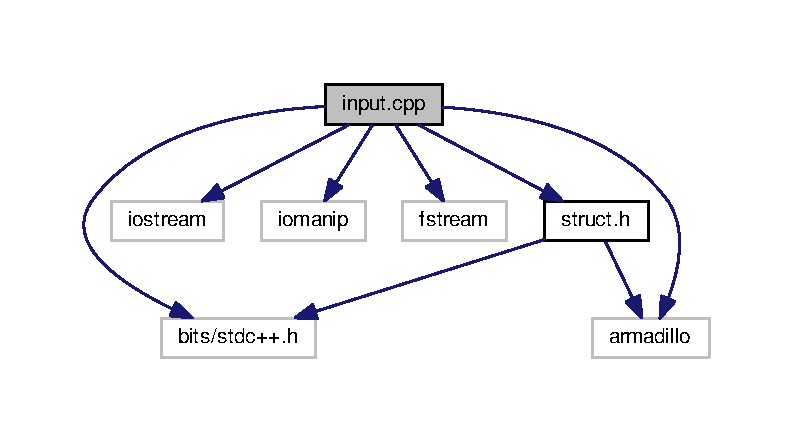
\includegraphics[width=350pt]{input_8cpp__incl}
\end{center}
\end{figure}
This graph shows which files directly or indirectly include this file\+:
\nopagebreak
\begin{figure}[H]
\begin{center}
\leavevmode
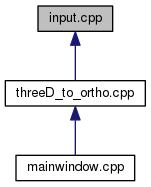
\includegraphics[width=185pt]{input_8cpp__dep__incl}
\end{center}
\end{figure}
\subsection*{Functions}
\begin{DoxyCompactItemize}
\item 
graph \hyperlink{input_8cpp_a0cc06af05bb805fba84d372efc4c247e}{get\+\_\+3\+D\+\_\+graph} (string filename=\char`\"{}input\+\_\+3\+D.\+txt\char`\"{})
\item 
mat \hyperlink{input_8cpp_a80d750ad6a6d88be3e402910c4e7438d}{get\+\_\+mx4\+\_\+matrix} (vector$<$ node $>$ v, int cols=4)
\end{DoxyCompactItemize}


\subsection{Function Documentation}
\mbox{\Hypertarget{input_8cpp_a0cc06af05bb805fba84d372efc4c247e}\label{input_8cpp_a0cc06af05bb805fba84d372efc4c247e}} 
\index{input.\+cpp@{input.\+cpp}!get\+\_\+3\+D\+\_\+graph@{get\+\_\+3\+D\+\_\+graph}}
\index{get\+\_\+3\+D\+\_\+graph@{get\+\_\+3\+D\+\_\+graph}!input.\+cpp@{input.\+cpp}}
\subsubsection{\texorpdfstring{get\+\_\+3\+D\+\_\+graph()}{get\_3D\_graph()}}
{\footnotesize\ttfamily graph get\+\_\+3\+D\+\_\+graph (\begin{DoxyParamCaption}\item[{string}]{filename = {\ttfamily \char`\"{}input\+\_\+3D.txt\char`\"{}} }\end{DoxyParamCaption})}

Reads the 3D input from a file given as an argument. Converts the input into a graph and returns the graph.\mbox{\Hypertarget{input_8cpp_a80d750ad6a6d88be3e402910c4e7438d}\label{input_8cpp_a80d750ad6a6d88be3e402910c4e7438d}} 
\index{input.\+cpp@{input.\+cpp}!get\+\_\+mx4\+\_\+matrix@{get\+\_\+mx4\+\_\+matrix}}
\index{get\+\_\+mx4\+\_\+matrix@{get\+\_\+mx4\+\_\+matrix}!input.\+cpp@{input.\+cpp}}
\subsubsection{\texorpdfstring{get\+\_\+mx4\+\_\+matrix()}{get\_mx4\_matrix()}}
{\footnotesize\ttfamily mat get\+\_\+mx4\+\_\+matrix (\begin{DoxyParamCaption}\item[{vector$<$ node $>$}]{v,  }\item[{int}]{cols = {\ttfamily 4} }\end{DoxyParamCaption})}

Takes a graph as an input. Converts the graph into a 4\+X4 coordinate matrix as specified in the mathematical model.
\hypertarget{matrices_8cpp}{}\section{matrices.\+cpp File Reference}
\label{matrices_8cpp}\index{matrices.\+cpp@{matrices.\+cpp}}
{\ttfamily \#include $<$bits/stdc++.\+h$>$}\newline
Include dependency graph for matrices.\+cpp\+:
% FIG 0
\subsection*{Classes}
\begin{DoxyCompactItemize}
\item 
class \hyperlink{classmatrices}{matrices}
\end{DoxyCompactItemize}

\hypertarget{Output_8cpp}{}\section{Output.\+cpp File Reference}
\label{Output_8cpp}\index{Output.\+cpp@{Output.\+cpp}}
{\ttfamily \#include $<$bits/stdc++.\+h$>$}\newline
Include dependency graph for Output.\+cpp\+:
% FIG 0
\subsection*{Classes}
\begin{DoxyCompactItemize}
\item 
class \hyperlink{classOutput}{Output}
\end{DoxyCompactItemize}

\hypertarget{readme_8md}{}\section{readme.\+md File Reference}
\label{readme_8md}\index{readme.\+md@{readme.\+md}}

\hypertarget{README_8md}{}\section{R\+E\+A\+D\+M\+E.\+md File Reference}
\label{README_8md}\index{R\+E\+A\+D\+M\+E.\+md@{R\+E\+A\+D\+M\+E.\+md}}

\hypertarget{threeD__to__ortho_8cpp}{}\section{three\+D\+\_\+to\+\_\+ortho.\+cpp File Reference}
\label{threeD__to__ortho_8cpp}\index{three\+D\+\_\+to\+\_\+ortho.\+cpp@{three\+D\+\_\+to\+\_\+ortho.\+cpp}}
{\ttfamily \#include $<$bits/stdc++.\+h$>$}\newline
{\ttfamily \#include $<$armadillo$>$}\newline
{\ttfamily \#include \char`\"{}input.\+cpp\char`\"{}}\newline
{\ttfamily \#include $<$math.\+h$>$}\newline
Include dependency graph for three\+D\+\_\+to\+\_\+ortho.\+cpp\+:
\nopagebreak
\begin{figure}[H]
\begin{center}
\leavevmode
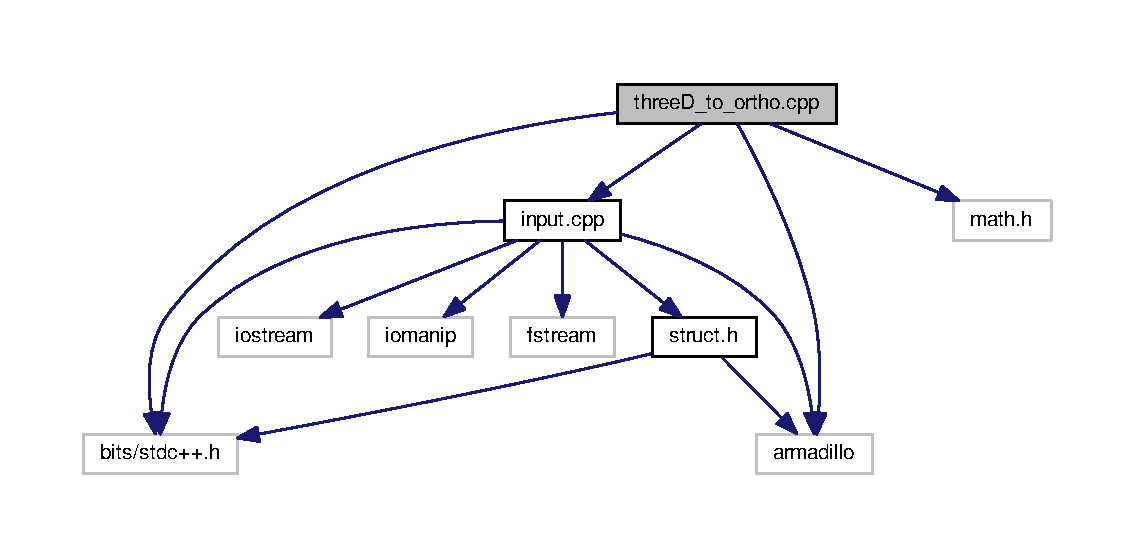
\includegraphics[width=350pt]{threeD__to__ortho_8cpp__incl}
\end{center}
\end{figure}
This graph shows which files directly or indirectly include this file\+:
\nopagebreak
\begin{figure}[H]
\begin{center}
\leavevmode
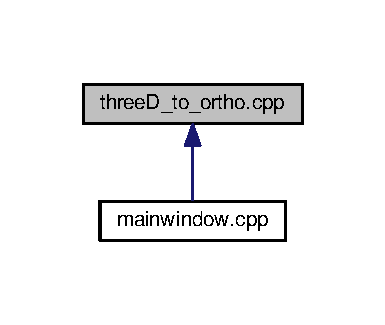
\includegraphics[width=185pt]{threeD__to__ortho_8cpp__dep__incl}
\end{center}
\end{figure}
\subsection*{Macros}
\begin{DoxyCompactItemize}
\item 
\#define \hyperlink{threeD__to__ortho_8cpp_a598a3330b3c21701223ee0ca14316eca}{PI}~3.\+1415926536
\end{DoxyCompactItemize}
\subsection*{Functions}
\begin{DoxyCompactItemize}
\item 
\hyperlink{structdir__ratios}{dir\+\_\+ratios} \hyperlink{threeD__to__ortho_8cpp_a42f9a16ee1fb5f0b3db37d7025ae8fb4}{get\+\_\+dir\+\_\+ratios} ()
\item 
mat \hyperlink{threeD__to__ortho_8cpp_a8420d58e0454a5d63fdb1d74ef96d270}{graph\+\_\+to\+\_\+mat} (vector$<$ \hyperlink{structnode}{node} $>$ nodes, int cols=4)
\item 
vector$<$ \hyperlink{structnode}{node} $>$ \hyperlink{threeD__to__ortho_8cpp_a6293222d57d26a387793e397a0418b31}{mat\+\_\+to\+\_\+graph} (mat A, vector$<$ \hyperlink{structnode}{node} $>$ vec)
\item 
mat \hyperlink{threeD__to__ortho_8cpp_a0f52d843a3641070bfa5443bcc3966d7}{translate\+\_\+graph} (mat A, \hyperlink{structcoordinate}{coordinate} t\+\_\+factor)
\item 
\hyperlink{structrot__matrix}{rot\+\_\+matrix} \hyperlink{threeD__to__ortho_8cpp_a221fd906c7bf89ca0a820709d0734f23}{rot\+\_\+about\+\_\+coord\+\_\+axis} (\hyperlink{structdirection}{direction} theta)
\item 
mat \hyperlink{threeD__to__ortho_8cpp_acd70b7328b74ddc50dc03870b7e3a6ed}{find\+\_\+rot} (mat A, \hyperlink{structdir__ratios}{dir\+\_\+ratios} d)
\item 
mat \hyperlink{threeD__to__ortho_8cpp_a50ff42487e337cc300dddef30e476cc0}{find\+\_\+projection} (mat A)
\item 
vector$<$ \hyperlink{structnode}{node} $>$ \hyperlink{threeD__to__ortho_8cpp_a3ced4e2119422236523faa8fcdd68acb}{find\+\_\+ortho} (vector$<$ \hyperlink{structnode}{node} $>$ \hyperlink{structgraph}{graph})
\item 
void \hyperlink{threeD__to__ortho_8cpp_a87e17a4e0a3335783284b821f184a923}{rotate\+\_\+graph} (vector$<$ \hyperlink{structnode}{node} $>$ \&v, \hyperlink{structdirection}{direction} theta, int x, int y, int z)
\end{DoxyCompactItemize}


\subsection{Macro Definition Documentation}
\mbox{\Hypertarget{threeD__to__ortho_8cpp_a598a3330b3c21701223ee0ca14316eca}\label{threeD__to__ortho_8cpp_a598a3330b3c21701223ee0ca14316eca}} 
\index{three\+D\+\_\+to\+\_\+ortho.\+cpp@{three\+D\+\_\+to\+\_\+ortho.\+cpp}!PI@{PI}}
\index{PI@{PI}!three\+D\+\_\+to\+\_\+ortho.\+cpp@{three\+D\+\_\+to\+\_\+ortho.\+cpp}}
\subsubsection{\texorpdfstring{PI}{PI}}
{\footnotesize\ttfamily \#define PI~3.\+1415926536}



\subsection{Function Documentation}
\mbox{\Hypertarget{threeD__to__ortho_8cpp_a3ced4e2119422236523faa8fcdd68acb}\label{threeD__to__ortho_8cpp_a3ced4e2119422236523faa8fcdd68acb}} 
\index{three\+D\+\_\+to\+\_\+ortho.\+cpp@{three\+D\+\_\+to\+\_\+ortho.\+cpp}!find\+\_\+ortho@{find\+\_\+ortho}}
\index{find\+\_\+ortho@{find\+\_\+ortho}!three\+D\+\_\+to\+\_\+ortho.\+cpp@{three\+D\+\_\+to\+\_\+ortho.\+cpp}}
\subsubsection{\texorpdfstring{find\+\_\+ortho()}{find\_ortho()}}
{\footnotesize\ttfamily vector$<$\hyperlink{structnode}{node}$>$ find\+\_\+ortho (\begin{DoxyParamCaption}\item[{vector$<$ \hyperlink{structnode}{node} $>$}]{graph }\end{DoxyParamCaption})}

Takes the graph whose projection is required to be taken as an argument. Then asks the user about the direction ratios of the desired line of sight. Then converts the graph to a matrix. Finds the transitions to be done. Applies the transitions to the coordinate matrx. Converts the matrix back to a graph and returns it.\mbox{\Hypertarget{threeD__to__ortho_8cpp_a50ff42487e337cc300dddef30e476cc0}\label{threeD__to__ortho_8cpp_a50ff42487e337cc300dddef30e476cc0}} 
\index{three\+D\+\_\+to\+\_\+ortho.\+cpp@{three\+D\+\_\+to\+\_\+ortho.\+cpp}!find\+\_\+projection@{find\+\_\+projection}}
\index{find\+\_\+projection@{find\+\_\+projection}!three\+D\+\_\+to\+\_\+ortho.\+cpp@{three\+D\+\_\+to\+\_\+ortho.\+cpp}}
\subsubsection{\texorpdfstring{find\+\_\+projection()}{find\_projection()}}
{\footnotesize\ttfamily mat find\+\_\+projection (\begin{DoxyParamCaption}\item[{mat}]{A }\end{DoxyParamCaption})}

Returns the projection of the graph after applying all the required transitions using z axis as the line-\/of-\/sight.\mbox{\Hypertarget{threeD__to__ortho_8cpp_acd70b7328b74ddc50dc03870b7e3a6ed}\label{threeD__to__ortho_8cpp_acd70b7328b74ddc50dc03870b7e3a6ed}} 
\index{three\+D\+\_\+to\+\_\+ortho.\+cpp@{three\+D\+\_\+to\+\_\+ortho.\+cpp}!find\+\_\+rot@{find\+\_\+rot}}
\index{find\+\_\+rot@{find\+\_\+rot}!three\+D\+\_\+to\+\_\+ortho.\+cpp@{three\+D\+\_\+to\+\_\+ortho.\+cpp}}
\subsubsection{\texorpdfstring{find\+\_\+rot()}{find\_rot()}}
{\footnotesize\ttfamily mat find\+\_\+rot (\begin{DoxyParamCaption}\item[{mat}]{A,  }\item[{\hyperlink{structdir__ratios}{dir\+\_\+ratios}}]{d }\end{DoxyParamCaption})}

Takes two inputs
\begin{DoxyItemize}
\item The matrix A which has to translated
\item The direction ratios of the direction which has to become the line of sight for taking the projections. This function calls the function rot\+\_\+about\+\_\+coord\+\_\+axis to get the rotation matrices and then multiplies the matrices with the coordinate matrix. It returns the coordinate matrix after multiplying it with the rotation matrices.
\end{DoxyItemize}\mbox{\Hypertarget{threeD__to__ortho_8cpp_a42f9a16ee1fb5f0b3db37d7025ae8fb4}\label{threeD__to__ortho_8cpp_a42f9a16ee1fb5f0b3db37d7025ae8fb4}} 
\index{three\+D\+\_\+to\+\_\+ortho.\+cpp@{three\+D\+\_\+to\+\_\+ortho.\+cpp}!get\+\_\+dir\+\_\+ratios@{get\+\_\+dir\+\_\+ratios}}
\index{get\+\_\+dir\+\_\+ratios@{get\+\_\+dir\+\_\+ratios}!three\+D\+\_\+to\+\_\+ortho.\+cpp@{three\+D\+\_\+to\+\_\+ortho.\+cpp}}
\subsubsection{\texorpdfstring{get\+\_\+dir\+\_\+ratios()}{get\_dir\_ratios()}}
{\footnotesize\ttfamily \hyperlink{structdir__ratios}{dir\+\_\+ratios} get\+\_\+dir\+\_\+ratios (\begin{DoxyParamCaption}{ }\end{DoxyParamCaption})}

Asks the user for the direction along which it is desired to take the projection.\mbox{\Hypertarget{threeD__to__ortho_8cpp_a8420d58e0454a5d63fdb1d74ef96d270}\label{threeD__to__ortho_8cpp_a8420d58e0454a5d63fdb1d74ef96d270}} 
\index{three\+D\+\_\+to\+\_\+ortho.\+cpp@{three\+D\+\_\+to\+\_\+ortho.\+cpp}!graph\+\_\+to\+\_\+mat@{graph\+\_\+to\+\_\+mat}}
\index{graph\+\_\+to\+\_\+mat@{graph\+\_\+to\+\_\+mat}!three\+D\+\_\+to\+\_\+ortho.\+cpp@{three\+D\+\_\+to\+\_\+ortho.\+cpp}}
\subsubsection{\texorpdfstring{graph\+\_\+to\+\_\+mat()}{graph\_to\_mat()}}
{\footnotesize\ttfamily mat graph\+\_\+to\+\_\+mat (\begin{DoxyParamCaption}\item[{vector$<$ \hyperlink{structnode}{node} $>$}]{nodes,  }\item[{int}]{cols = {\ttfamily 4} }\end{DoxyParamCaption})}

Takes a graph as an input. Converts the graph into a 4\+X4 coordinate matrix as specified in the mathematical model.\mbox{\Hypertarget{threeD__to__ortho_8cpp_a6293222d57d26a387793e397a0418b31}\label{threeD__to__ortho_8cpp_a6293222d57d26a387793e397a0418b31}} 
\index{three\+D\+\_\+to\+\_\+ortho.\+cpp@{three\+D\+\_\+to\+\_\+ortho.\+cpp}!mat\+\_\+to\+\_\+graph@{mat\+\_\+to\+\_\+graph}}
\index{mat\+\_\+to\+\_\+graph@{mat\+\_\+to\+\_\+graph}!three\+D\+\_\+to\+\_\+ortho.\+cpp@{three\+D\+\_\+to\+\_\+ortho.\+cpp}}
\subsubsection{\texorpdfstring{mat\+\_\+to\+\_\+graph()}{mat\_to\_graph()}}
{\footnotesize\ttfamily vector$<$\hyperlink{structnode}{node}$>$ mat\+\_\+to\+\_\+graph (\begin{DoxyParamCaption}\item[{mat}]{A,  }\item[{vector$<$ \hyperlink{structnode}{node} $>$}]{vec }\end{DoxyParamCaption})}

Takes a coordinate matrix as an input. Converts 4\+X4 coordinate matrix to the graph which would lead to constriuction of this matrix.\mbox{\Hypertarget{threeD__to__ortho_8cpp_a221fd906c7bf89ca0a820709d0734f23}\label{threeD__to__ortho_8cpp_a221fd906c7bf89ca0a820709d0734f23}} 
\index{three\+D\+\_\+to\+\_\+ortho.\+cpp@{three\+D\+\_\+to\+\_\+ortho.\+cpp}!rot\+\_\+about\+\_\+coord\+\_\+axis@{rot\+\_\+about\+\_\+coord\+\_\+axis}}
\index{rot\+\_\+about\+\_\+coord\+\_\+axis@{rot\+\_\+about\+\_\+coord\+\_\+axis}!three\+D\+\_\+to\+\_\+ortho.\+cpp@{three\+D\+\_\+to\+\_\+ortho.\+cpp}}
\subsubsection{\texorpdfstring{rot\+\_\+about\+\_\+coord\+\_\+axis()}{rot\_about\_coord\_axis()}}
{\footnotesize\ttfamily \hyperlink{structrot__matrix}{rot\+\_\+matrix} rot\+\_\+about\+\_\+coord\+\_\+axis (\begin{DoxyParamCaption}\item[{\hyperlink{structdirection}{direction}}]{theta }\end{DoxyParamCaption})}

Takes the direction ratios as the input It returns the rotation matrices which are to be multiplied to the coordinate matrix so as to make the Z axis coincide with the given direction theta. It returns a struct of \hyperlink{structrot__matrix}{rot\+\_\+matrix} type which contains the three rotation matrices namely Rx, Ry and Rz.\mbox{\Hypertarget{threeD__to__ortho_8cpp_a87e17a4e0a3335783284b821f184a923}\label{threeD__to__ortho_8cpp_a87e17a4e0a3335783284b821f184a923}} 
\index{three\+D\+\_\+to\+\_\+ortho.\+cpp@{three\+D\+\_\+to\+\_\+ortho.\+cpp}!rotate\+\_\+graph@{rotate\+\_\+graph}}
\index{rotate\+\_\+graph@{rotate\+\_\+graph}!three\+D\+\_\+to\+\_\+ortho.\+cpp@{three\+D\+\_\+to\+\_\+ortho.\+cpp}}
\subsubsection{\texorpdfstring{rotate\+\_\+graph()}{rotate\_graph()}}
{\footnotesize\ttfamily void rotate\+\_\+graph (\begin{DoxyParamCaption}\item[{vector$<$ \hyperlink{structnode}{node} $>$ \&}]{v,  }\item[{\hyperlink{structdirection}{direction}}]{theta,  }\item[{int}]{x,  }\item[{int}]{y,  }\item[{int}]{z }\end{DoxyParamCaption})}

Rotate the given graph about axis (X, Y or Z axis) depending on the input x, y and z Finsd the rotations matrix for the given direction theta and applies only those whose corresponding input is 1. For Rx, x is to be 1. For Ry, y is to be 1. For Rz, z is to be 1.\mbox{\Hypertarget{threeD__to__ortho_8cpp_a0f52d843a3641070bfa5443bcc3966d7}\label{threeD__to__ortho_8cpp_a0f52d843a3641070bfa5443bcc3966d7}} 
\index{three\+D\+\_\+to\+\_\+ortho.\+cpp@{three\+D\+\_\+to\+\_\+ortho.\+cpp}!translate\+\_\+graph@{translate\+\_\+graph}}
\index{translate\+\_\+graph@{translate\+\_\+graph}!three\+D\+\_\+to\+\_\+ortho.\+cpp@{three\+D\+\_\+to\+\_\+ortho.\+cpp}}
\subsubsection{\texorpdfstring{translate\+\_\+graph()}{translate\_graph()}}
{\footnotesize\ttfamily mat translate\+\_\+graph (\begin{DoxyParamCaption}\item[{mat}]{A,  }\item[{\hyperlink{structcoordinate}{coordinate}}]{t\+\_\+factor }\end{DoxyParamCaption})}

Takes two inputs
\begin{DoxyItemize}
\item The matrix A (for the corresponding graph) which has to translated
\item The coordinate t\+\_\+factor of the point that would become the origin in the translated system. This function makes multiple calls to the function translate\+\_\+coordinate for all the vertices of the input graph.
\end{DoxyItemize}
\hypertarget{twoD__to__threeD_8cpp}{}\section{two\+D\+\_\+to\+\_\+three\+D.\+cpp File Reference}
\label{twoD__to__threeD_8cpp}\index{two\+D\+\_\+to\+\_\+three\+D.\+cpp@{two\+D\+\_\+to\+\_\+three\+D.\+cpp}}
{\ttfamily \#include $<$bits/stdc++.\+h$>$}\newline
{\ttfamily \#include $<$input.\+cpp$>$}\newline
Include dependency graph for two\+D\+\_\+to\+\_\+three\+D.\+cpp\+:
% FIG 0
\subsection*{Classes}
\begin{DoxyCompactItemize}
\item 
class \hyperlink{classtwoD__to__threeD}{two\+D\+\_\+to\+\_\+threeD}
\end{DoxyCompactItemize}

%--- End generated contents ---

% Index
\backmatter
\newpage
\phantomsection
\clearemptydoublepage
\addcontentsline{toc}{chapter}{Index}
\printindex

\end{document}
